\section{Compilar G4mpi}

G4MPI es una interfaz nativa con bibliotecas MPI. El directorio contiene una biblioteca de IU de Geant4 y un par de ejemplos paralelizados. Con esta interfaz, las aplicaciones de los usuarios se pueden paralelizar con diferentes bibliotecas compatibles con MPI, como OpenMPI, LAM / MPI, MPICH2, etc.

\begin{figure}[H]
    \centering
  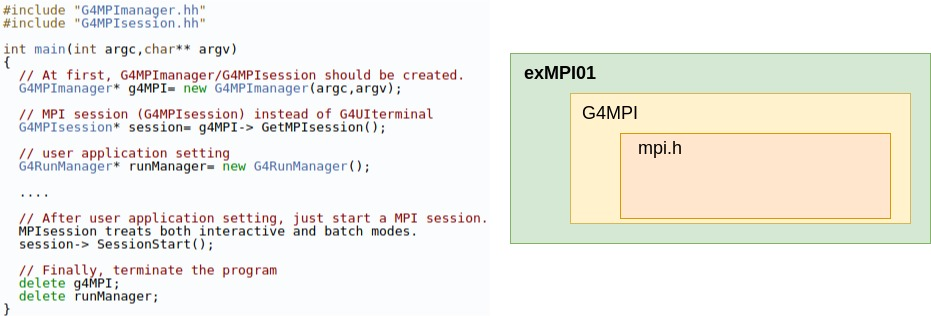
\includegraphics[width=0.7\textwidth]{images/estructure.jpg}
  \caption{Esquema}
  \label{esq}
\end{figure}

\subsection{Compilando G4mpi}


\begin{lstlisting}[language=bash,style=mystyle]   
mkdir build-mpi
cd build-mpi
cmake -DGeant4_DIR=/home/gfnun1/geant4/install/lib/Geant4-10.6.1 \
     -DCMAKE_INSTALL_PREFIX=/home/gfnun1/geant4/geant4-mpi \
     /home/gfnun1/geant4/src/geant4.10.06.p01/examples/extended/parallel/MPI/source
make
make install  
\end{lstlisting}


\subsection{Compilando Ejemplo exMP01}

\begin{lstlisting}[language=bash,style=mystyle]   
mkdir build
cd build
cmake -DG4mpi_DIR=<where-G4mpi-wasintalled>/lib[64]/G4mpi -DCMAKE_CXX_COMPILER=mpicxx \
      -DGeant4_DIR=<your Geant4 install path>/lib[64]/Geant4-V.m.n <path-to-source>
      (V.m.n is the version of Geant4, eg. Geant4-9.6.0)
make
make install
\end{lstlisting}

\begin{lstlisting}[language=bash,style=mystyle]
mkdir build
cd build
sudo cmake -DG4mpi_DIR=/home/gfnun/geant4/geant4-mpi/lib/G4mpi-10.6.1 -DCMAKE_CXX_COMPILER=mpicxx \
      -DGeant4_DIR=/home/gfnun/geant4/install/lib/Geant4-10.6.1 /home/gfnun1/geant4/src/geant4.10.06.p01/examples/extended/parallel/MPI/examples/exMPI01
make
make install 
\end{lstlisting}

\subsection{Ejecutando Ejemplo con open-mpi}

\begin{lstlisting}[language=bash,style=mystyle]
$ mpirun -np 3 --hostfile /home/gfnun1/my_hosts ./exMPI01
\end{lstlisting}

\newpage


